\documentclass[tikz]{standalone}


\usetikzlibrary{shapes.geometric, shapes.multipart, arrows, calc, through}


\begin{document}


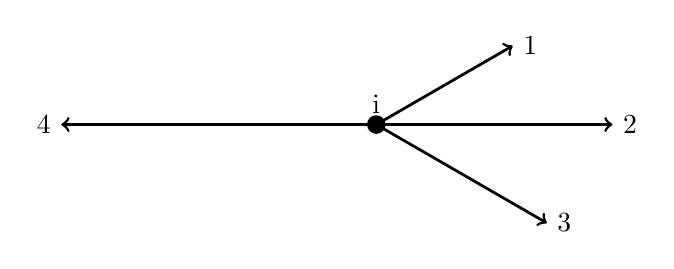
\begin{tikzpicture}[line width=1pt]
\draw[fill] (0,0)node[above]{i} circle[radius=0.1];
\draw[->](0,0)-- ++(30:2)node[right]{1};
\draw[->] (0,0) -- (3,0)node[right]{2};
\draw[->](0,0)-- ++(-30:2.5) node[right]{3};
\draw[->] (0,0) -- (-4,0)node[left]{4};
\end{tikzpicture}


\end{document}
